\documentclass[9pt]{extarticle}

\usepackage[utf8]{inputenc}
\usepackage[T1]{fontenc}
\usepackage{lmodern}
\usepackage{graphicx}
\usepackage{color}
\usepackage{hyperref}
\usepackage{amsmath}
\usepackage{amsfonts}
\usepackage{epstopdf}
\usepackage[table]{xcolor}
\usepackage[a4paper, total={6in, 10in}]{geometry}
\usepackage{enumitem}
\usepackage[export]{adjustbox}


\graphicspath{ {./Figures/} }


\begin{document}

{\huge Andrew Sivaprakasam | Cochlear Implant Project 2020 Write-up}

\section{Part A | Introduction to cochlear-implant signal processing}

\begin{enumerate}[label = \alph*) ]
\item Filter-bank reconstructions were generated using the \verb|quad_filt_bank.m| function from Delgutte within the \verb|get_Stimuli.m| function I created. The bands were set using the \verb|equal_xbm_bands.m| function. This function spaced the frequency bands to match the frequency distribution of the basilar membrane using Liberman's cat cochlear frequency map, scaling it to match the 22kHz hearing range of humans. For cochlear implant user simulation, this is important, since we assume cochlear implant electrodes (bands) are equally spaced. However, the frequency-specific IHCs in the cochlea are not equally spaced from 0-4 kHz, so this correction helps.  

\vspace{.5em}

Refer to \verb|B| in my \verb|get_Stimuli.m| code for the filter coefficients. 

\item Here are the envelope extractions visualized for the 1 band filter-bank. It is clear the Hilbert envelope is a lot more liberal than the 16 and 160 Hz envelope extraction methods, allowing it to capture a more detailed picture of the sound being played. 

\begin{center}
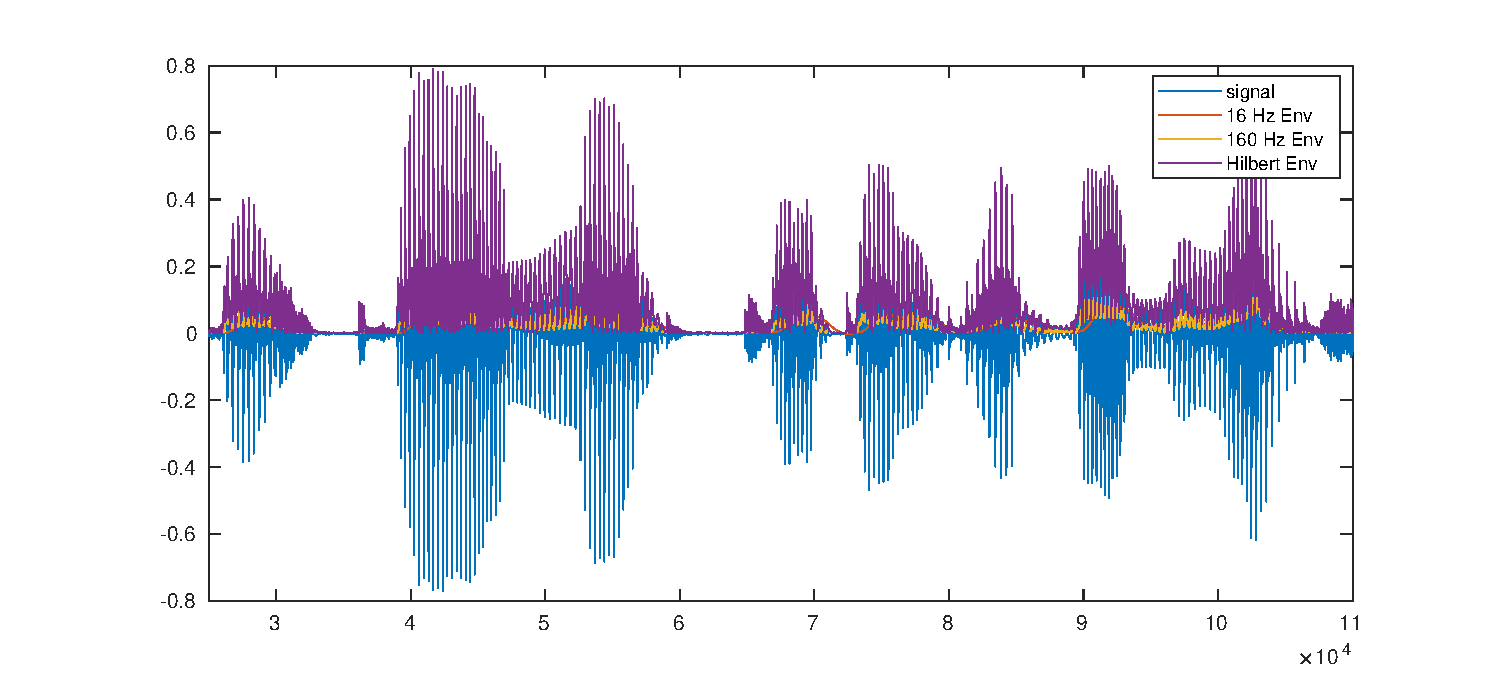
\includegraphics[width = .85\textwidth]{envelopes}
\end{center}

\item Here are some spectrograms (bandwidth 30 Hz, dynamic range 45 dB) that demonstrate proof of a working filter-bank: \\

\hspace{6.5em}\textbf{16 Hz} \hspace{11em} \textbf{160 Hz} \hspace{9em} \textbf{Hilbert}

\begin{center}
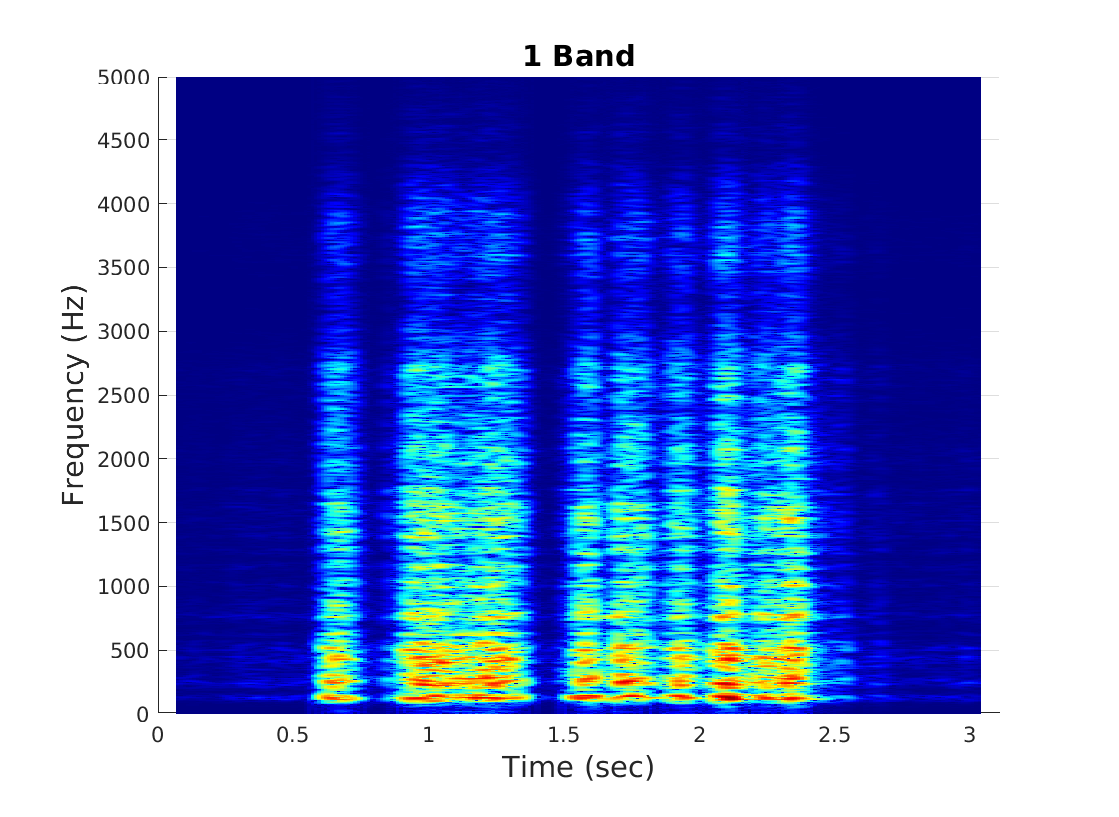
\includegraphics[width = .3\textwidth]{16_1}
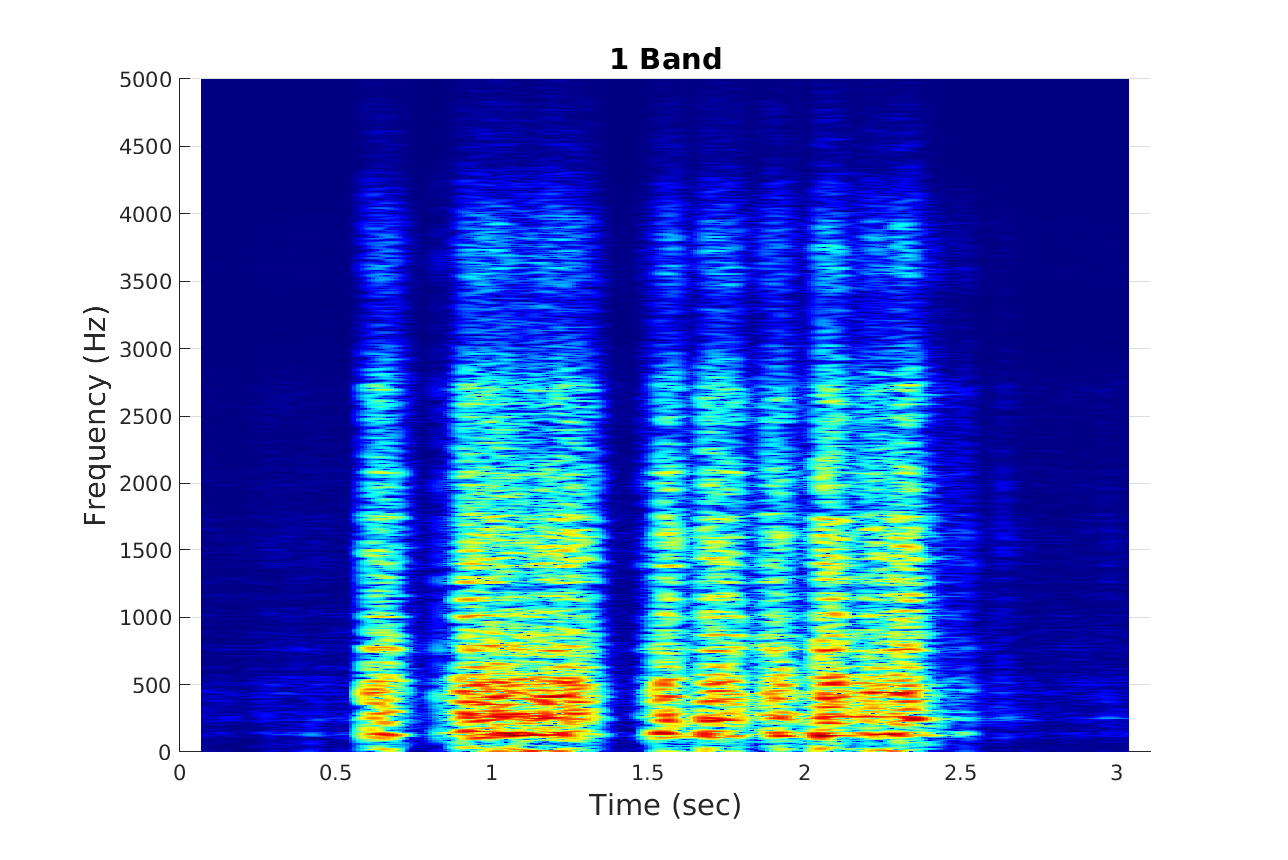
\includegraphics[width = .3\textwidth]{160_1}
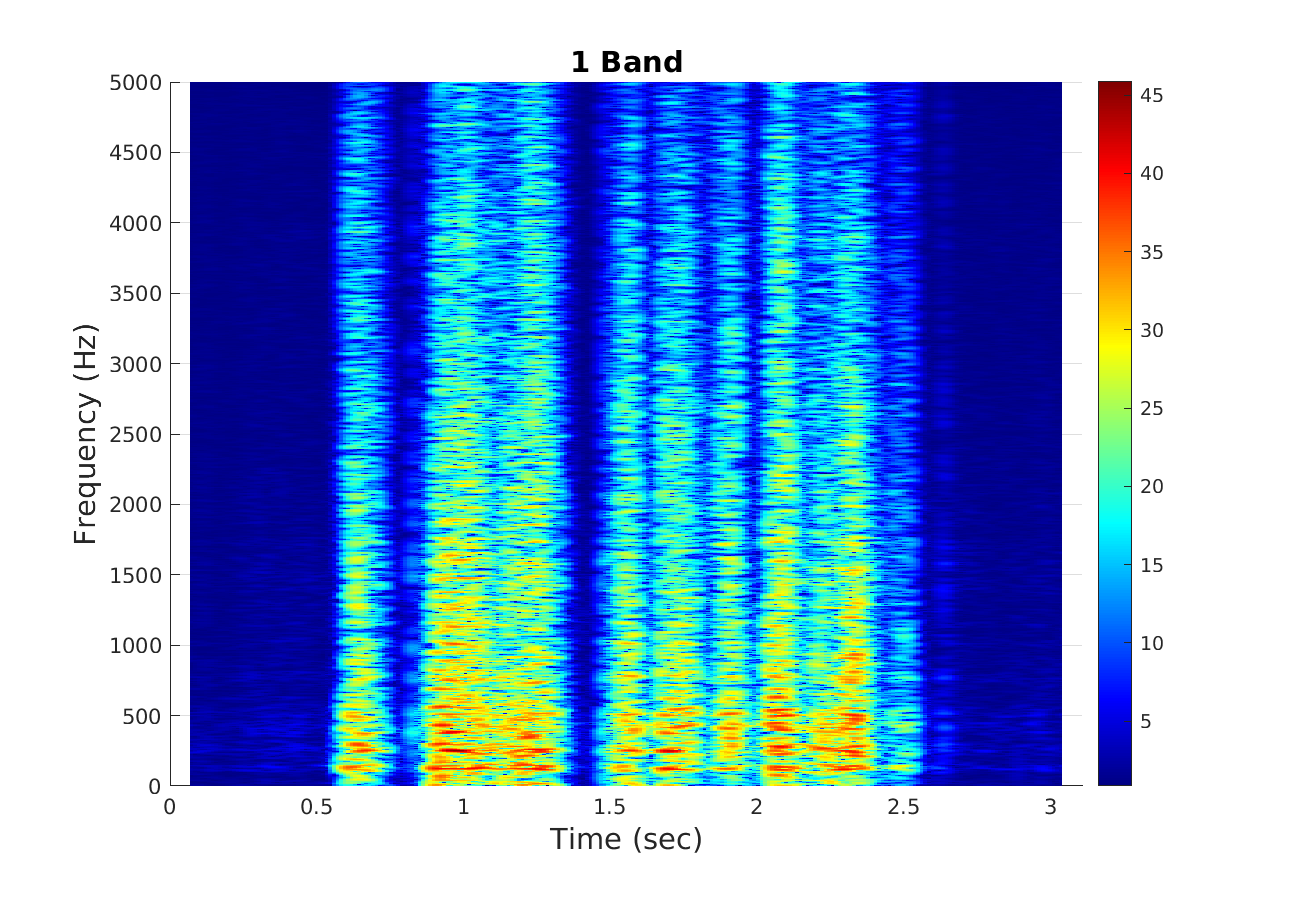
\includegraphics[width = .3\textwidth]{hilb_1} \\

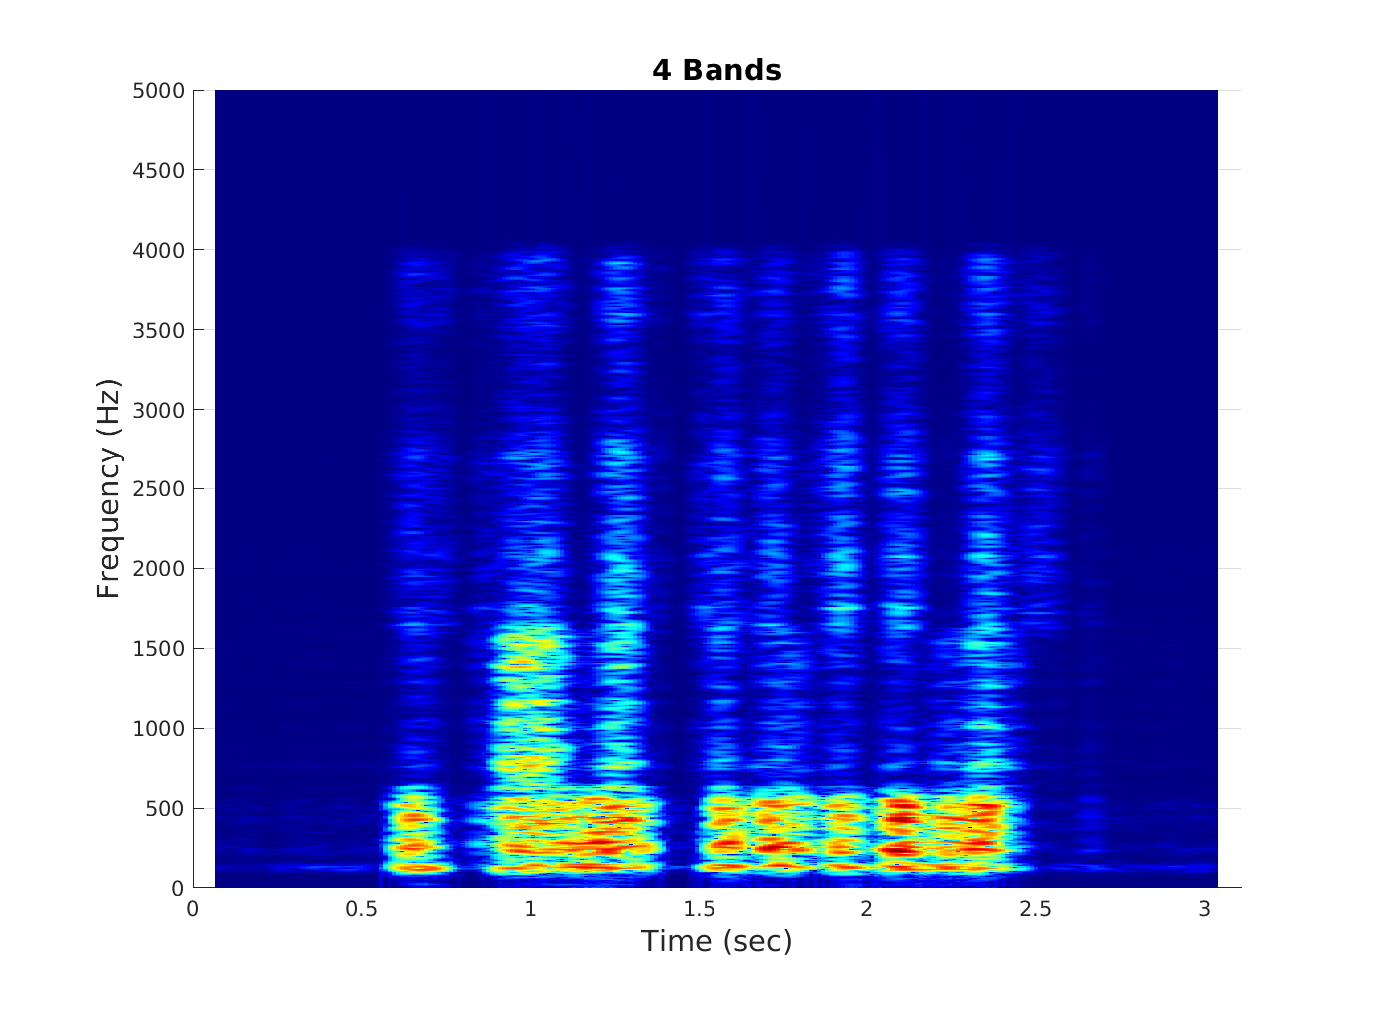
\includegraphics[width = .3\textwidth]{16_4}
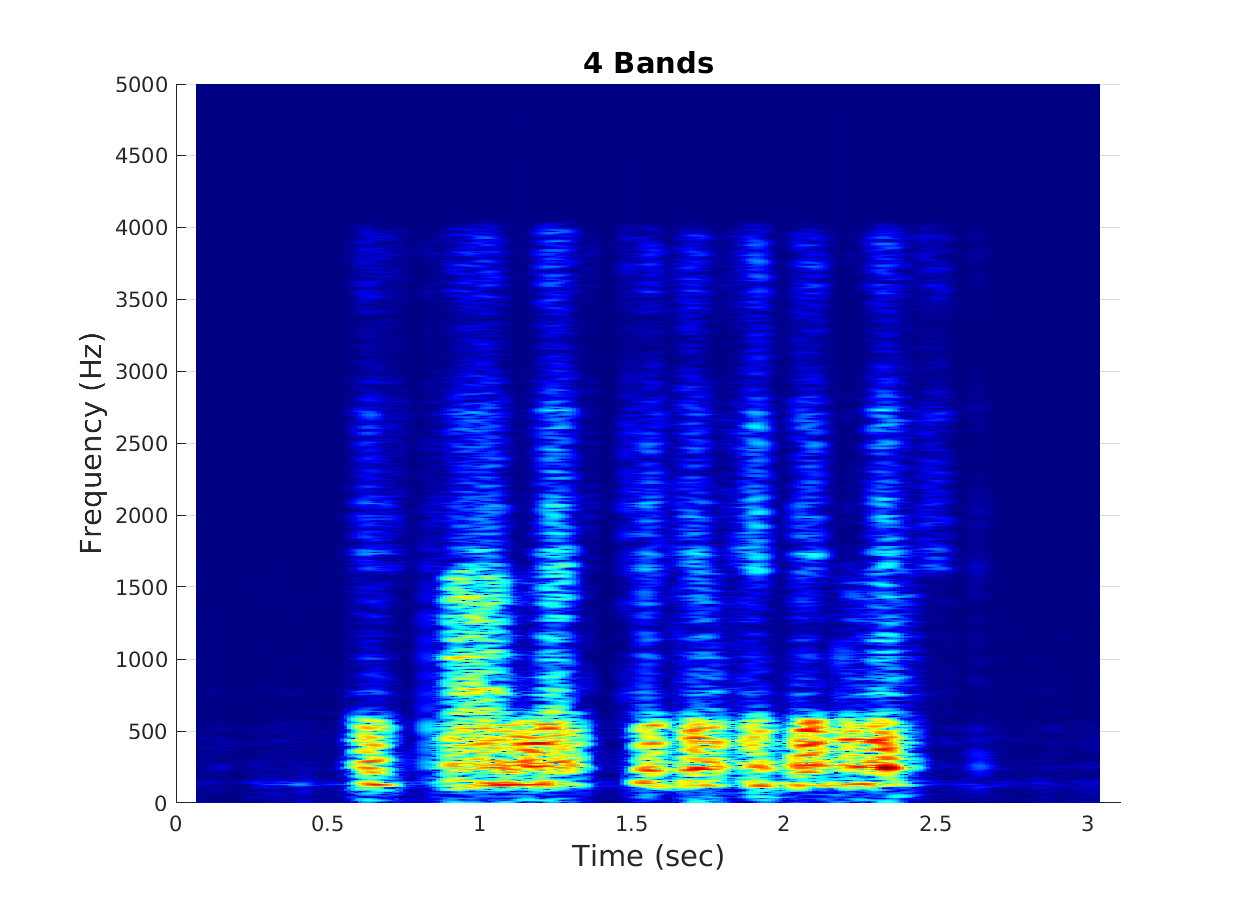
\includegraphics[width = .3\textwidth]{160_4}
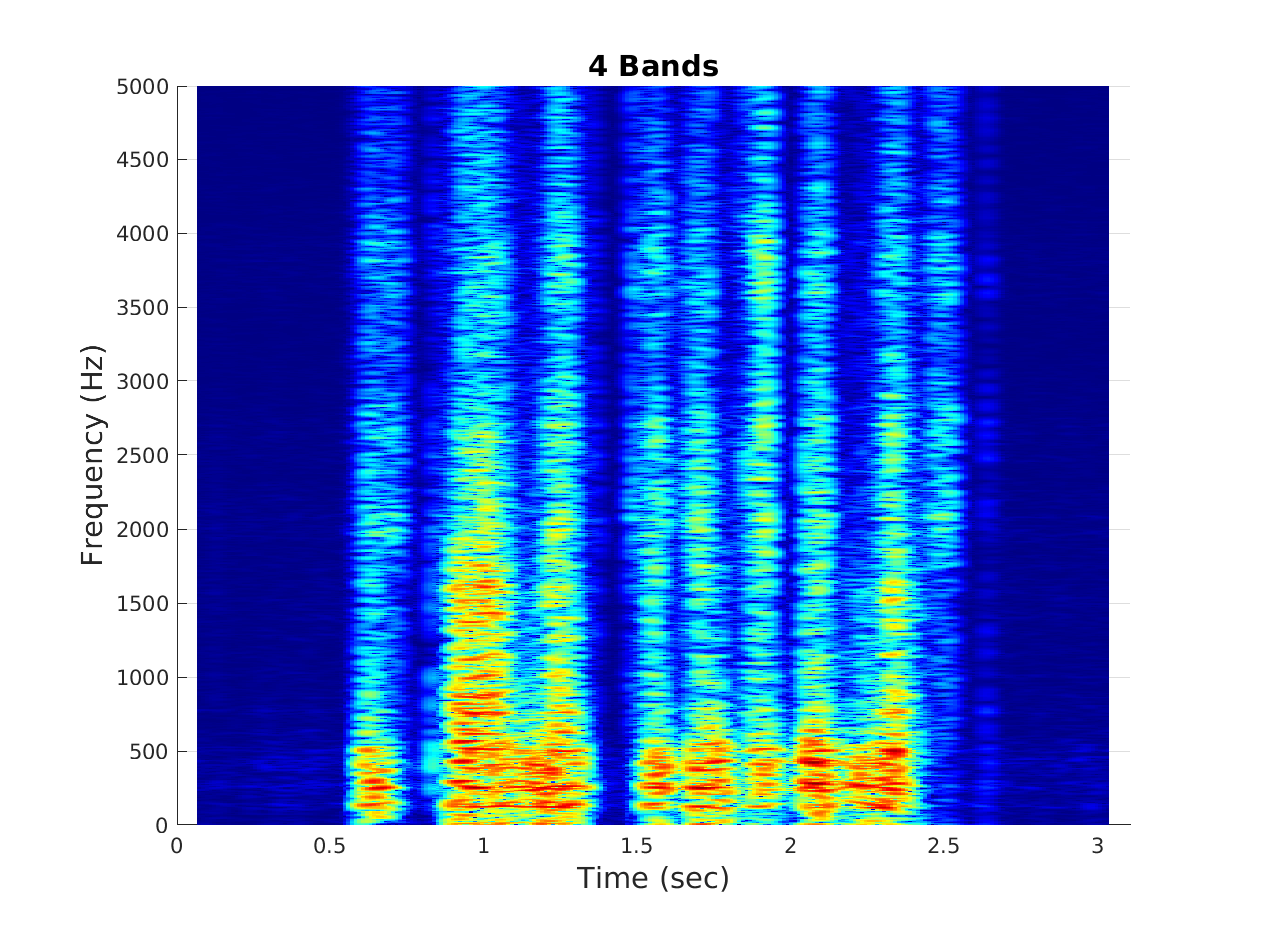
\includegraphics[width = .3\textwidth]{hilb_4} \\

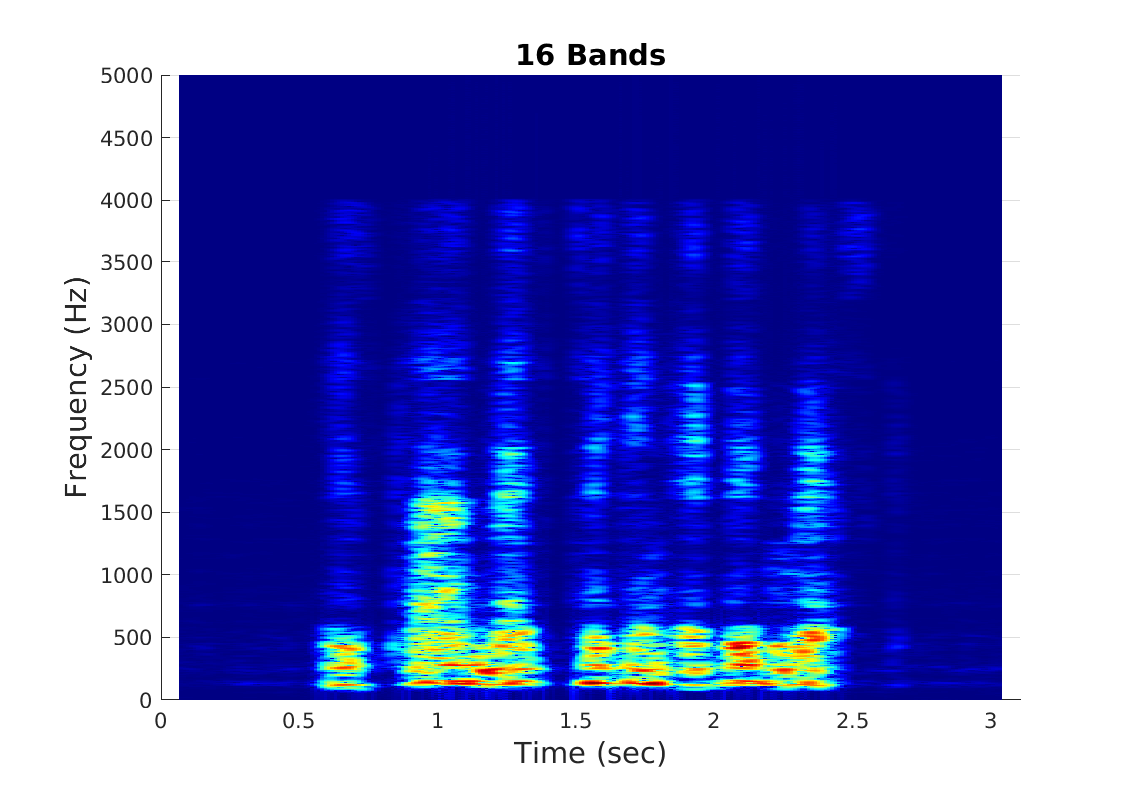
\includegraphics[width = .3\textwidth]{16_16}
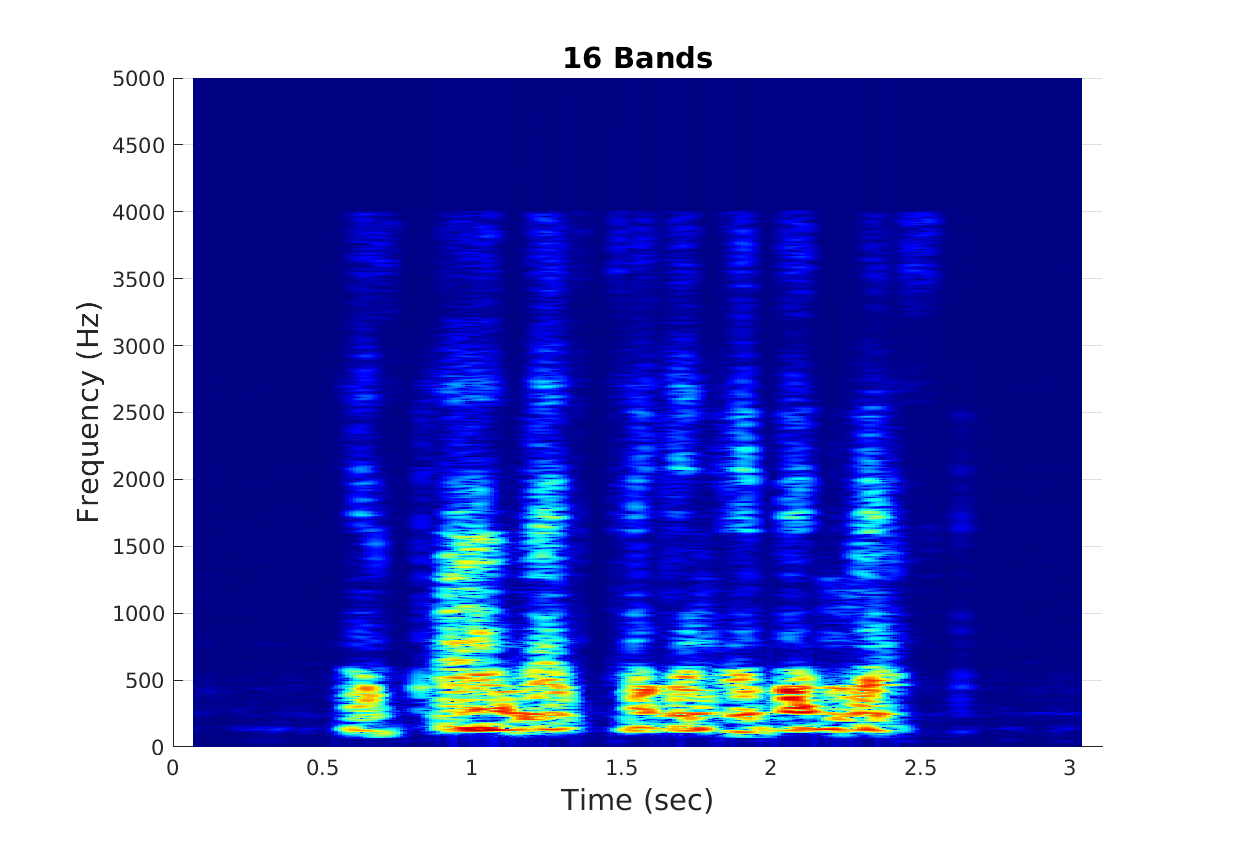
\includegraphics[width = .3\textwidth]{160_16}
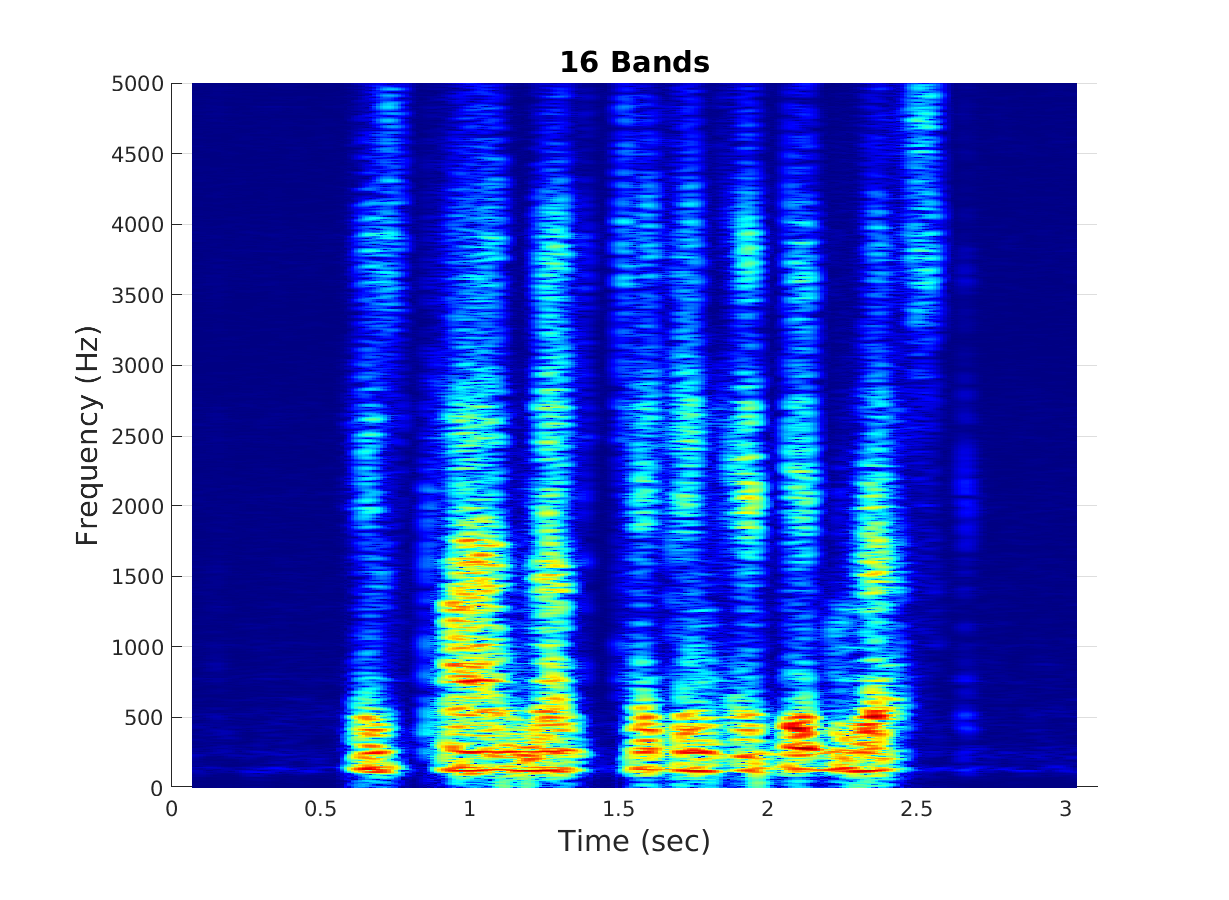
\includegraphics[width = .3\textwidth]{hilb_16} 
\end{center}

\newpage
The sharper cutoff at 4 kHz in the 16 and 160 Hz envelope extraction can be explained by the 4 kHz LPF filter I used  to emulate the Shannon et. al. (1995) study. Additionally, it is (again) clear that the Hilbert envelope extraction and presentation with a noise carrier captures more detail than the 16 and 160 Hz envelope extractions. All spectrograms tend to have closer representation of the raw recording as the number of bands increase. \textit{I apologize for these figures not being evenly sized. It's an eyesore but I had to get this done.}

\item The way we tested this was by taking ten of the SPIN-R sentences, and creating 16/160 Hz and Hilbert envelope extractions $\&$ noise carrier signal for all ten sentences. Our code then randomly presented these stimuli and asked the user to guess which sentence was presented. We presented a total of 120 sentences/subject. We tracked correctness, in addition to reaction time. The code for this may be found in \verb|runTrialA.m|. \\

From our results, it is clear that the Hilbert envelope allows for best representation of the sentence most-noticeably at the 1-2 Band filter-bank level. Above that, the 16/160 Hz envelope extraction works fairly well. It is important to consider the fact that our study was more primitive than the Shannon study. Instead of counting the number of words typed by the user, we went for a more simplistic approach to save time (10 alternative forced choice). Additionally, one of our subjects transcribed the sentences and de-bugged the code, so was rather familiar with the 10 sentences that were used, which results in better accuracy with sentence detection. \textbf{COMMENT ON 16 Hz vs others after Joe's results and mention our findings are similar to shannon!!!!} \\

Though our reaction time results are noisier and \textbf{don't demonstrate much variability between conditions}, they may demonstrate an increase in confidence of sentence identification as the number of bands increase. 

\begin{center}
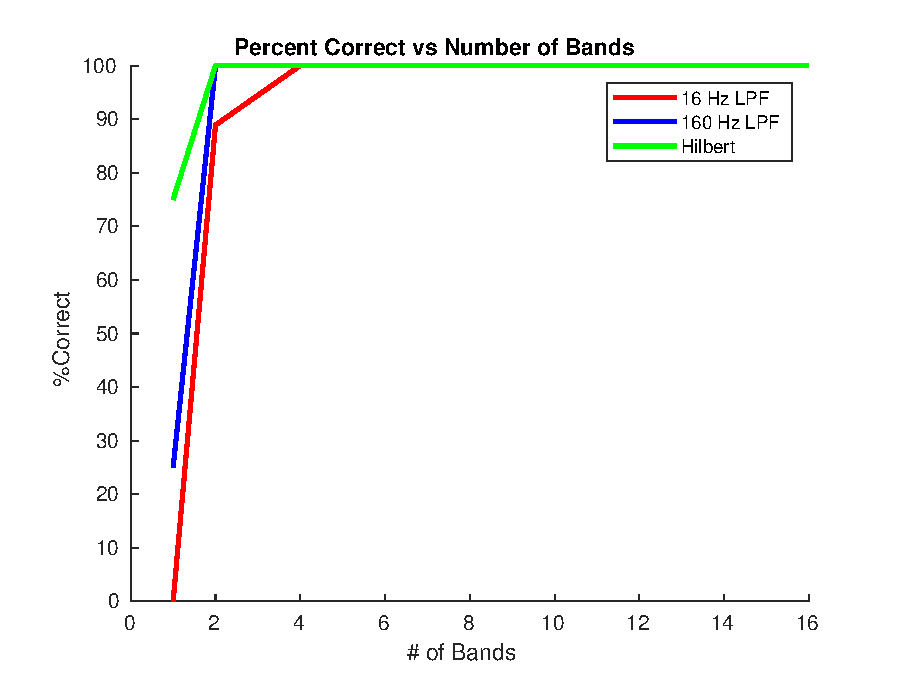
\includegraphics[width = .47\textwidth]{figA1}
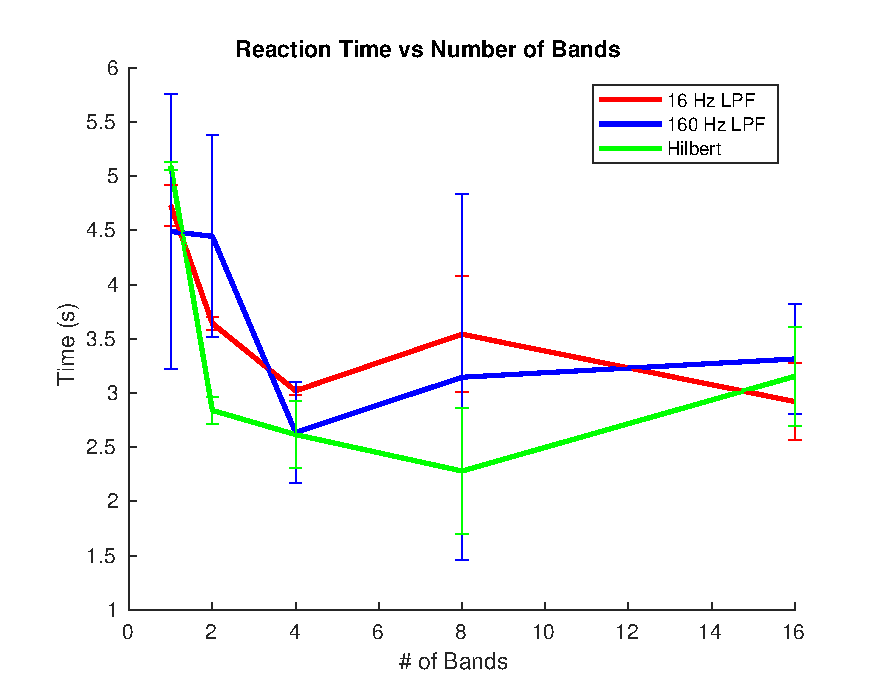
\includegraphics[width = .47\textwidth]{figA2}
\end{center}

\end{enumerate}


\section{Part B | Exploring potential for frequency modulation information to improve CI signal processing}

\begin{enumerate}[label = \alph*)]

\item asd

\end{enumerate}
\end{document}